

%% Hier schreibt man dann was. Und so \comment{kommentiert ihr Sachen.}. Offenbar sieht das nicht so schön aus.


%% \begin{figure}[ht]
%%   \subfloat[Pyramidenzelle \label{fig:pyramid_cell}]{%
%%     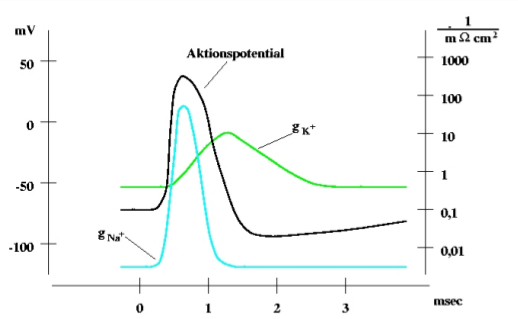
\includegraphics[width=0.4\linewidth]{aktionspotential}
%%   }
%%   \hfill
%%   \subfloat[Neocortex \label{fig:neocortex}]{%
%%     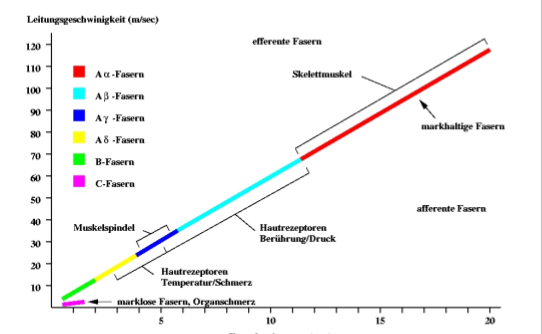
\includegraphics[width=0.5\textwidth]{leitungsgeschwindigkeit}
%%   }
%%   \caption[Aktionspotential und Leitungsgeschwindikeit]{Links:
%%     AP. Rechts: Leitungsgeschwindikeit von verschiedenen Fasern.}
%% \label{fig:ap_leitung}
%% \end{figure}



%%% Local Variables:
%%% mode: latex
%%% TeX-master: "../arbeit"
%%% End:
